
\section{Analisi dei risultati}

L'analisi \`e organizzata per esperimento. Si comincia dal primo perch\'e, oltre a fornire il costo
di riferimento, stabilisce \emph{quale grandezza} sia lecito usare come variabile di risposta: una
questione preliminare che condiziona la lettura di tutto il resto.

\subsection{Esperimento 1: la scelta della variabile di risposta}

Il generatore di carico riporta per ogni iterazione la durata della fase di lavoro e il periodo
osservato. Sarebbe naturale usare la prima come misura del costo della strumentazione. La
Figura~\ref{fig:07}, riquadro in basso a sinistra, mostra perch\'e ci\`o condurrebbe a una
conclusione falsa: il livello~1 di tracciamento risulta \textbf{pi\`u veloce} del livello 0, che
non esegue alcuna strumentazione. Poich\'e un overhead non pu\`o accelerare il codice, il risultato
\`e un artefatto.

\begin{figure}[h]\centering
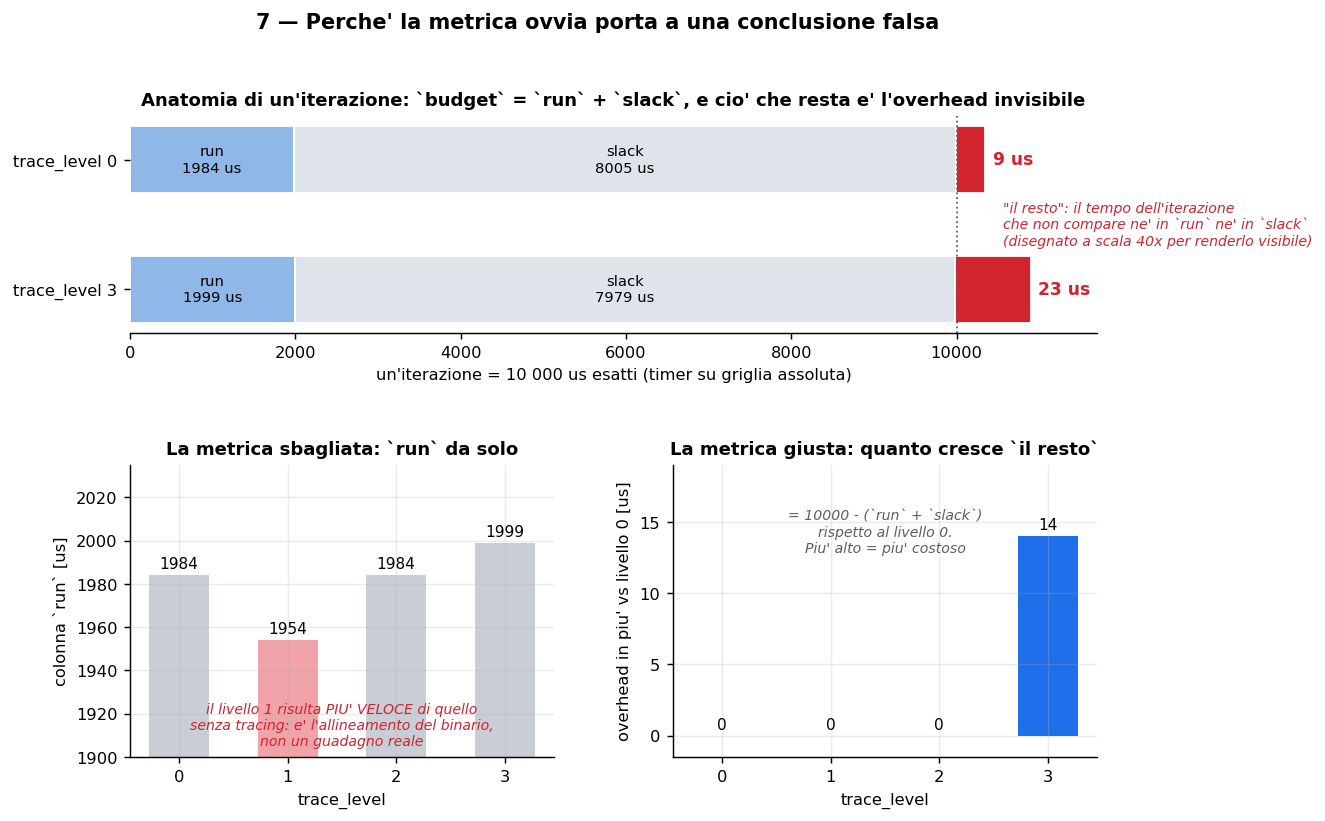
\includegraphics[width=\textwidth]{../2-DoE/figures/07_metric_artifact.png}
\caption{Anatomia di un'iterazione e confronto fra la grandezza riportata nativamente e quella
effettivamente indicativa del costo.}
\label{fig:07}
\end{figure}

La spiegazione richiede di guardare come si compone un'iterazione, riportata nel riquadro
superiore. Poich\'e il task critico si attiva su una griglia temporale fissa, fra due attivazioni
consecutive trascorrono esattamente 10\,000\us. Tale intervallo si ripartisce in tre contributi:

\begin{itemize}
\item la \textbf{fase di lavoro}, l'unica cronometrata esplicitamente;
\item il \textbf{margine residuo} rispetto alla scadenza, misurato al termine del lavoro;
\item la parte \textbf{non contabilizzata}, differenza fra il periodo e la somma delle due
precedenti, che comprende la latenza di risveglio, la scrittura del log e --- questo \`e il punto ---
la creazione e la chiusura degli elementi di traccia, che avvengono al di fuori della finestra
cronometrata.
\end{itemize}

Definiamo \emph{budget} la somma dei primi due contributi, cio\`e la porzione di iterazione che il
generatore misura. L'overhead della telemetria non compare in essa, ma nella terza: quanto pi\`u la
strumentazione lavora, tanto pi\`u il budget si riduce. L'ordinata del riquadro in basso a destra
riporta perci\`o di quanto cresce la parte non contabilizzata rispetto alla condizione senza
tracciamento.

\begin{table}[h]\centering\small
\begin{tabular}{cccccc}
\toprule
\textbf{livello} & fase di lavoro & margine residuo & \textbf{budget} & periodo & non contabilizzato \\
\midrule
0 & 1984 & 8005 & 9991 & 10\,000 & 9 \\
1 & 1954 & 8036 & 9991 & 10\,000 & 9 \\
2 & 1984 & 8006 & 9991 & 10\,000 & 9 \\
3 & 1999 & 7979 & 9977 & 10\,000 & \textbf{23} \\
\bottomrule
\end{tabular}
\caption{Scomposizione dell'iterazione per livello di tracciamento; valori in microsecondi,
mediane su 20 ripetizioni.}
\label{tab:anatomia}
\end{table}

La riga del livello~1 chiarisce l'artefatto. La fase di lavoro \emph{diminuisce} di 30\us{} rispetto
al livello 0, ma il margine residuo \emph{aumenta} di 31: i due si compensano e il budget resta
invariato. Se quei 30\us{} fossero stati lavoro realmente risparmiato, l'iterazione sarebbe
terminata prima e il margine sarebbe rimasto pi\`u ampio. Il tempo \`e semplicemente stato
contabilizzato altrove: eseguibili diversi dispongono il codice in memoria in modo leggermente
diverso, e la differenza di allineamento vale circa 30\us, cio\`e \textbf{pi\`u del segnale da
misurare}. Lo stesso vale per il periodo riportato, che al livello 3 risulta addirittura
\emph{pi\`u breve} proprio dove l'overhead cresce.

\textbf{Risultato.} Adottando il budget come variabile di risposta, i livelli 1 e 2 non producono
alcun effetto misurabile, mentre il livello 3 costa \textbf{circa 14\us{} per iterazione}: lo
0.14\,\% del periodo, ma lo 0.7\,\% del lavoro utile. Non si registra alcuna scadenza mancata a
nessun livello. La periodicit\`a non viene degradata: l'intervallo fra attivazioni consecutive resta
di 10\,000\us{} in tutte le condizioni.

\`E utile precisare che cosa \emph{non} rientra in quei 14\us. Scomponendo la parte non
contabilizzata mediante la latenza di risveglio, che il generatore registra separatamente, si
ottiene un contributo costante di circa 7.4\us{} dovuto al risveglio del thread e non attribuibile
alla telemetria; i restanti 14\us{} rappresentano il costo di \emph{costruire} gli elementi di
traccia, non di trasmetterli. La trasmissione, in questa configurazione, \`e a carico di un thread
separato: il suo costo emerger\`a nell'Esperimento 3.

\subsection{Esperimento 2: il campionamento non distingue le criticit\`a}

\`E il risultato centrale dello studio.

\begin{figure}[h]\centering
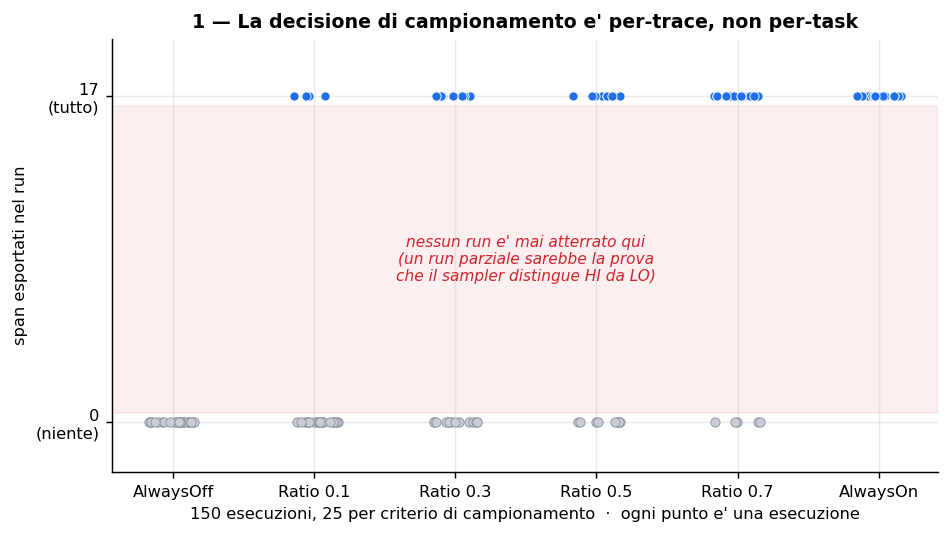
\includegraphics[width=\textwidth]{../2-DoE/figures/01_all_or_nothing.png}
\caption{Elementi di traccia emessi in ciascuna delle 150 esecuzioni, per criterio di
campionamento. La banda evidenziata copre tutti i valori intermedi.}
\label{fig:01}
\end{figure}

Nella Figura~\ref{fig:01} ogni punto rappresenta un'esecuzione. I punti si dispongono su due sole
righe: nessun elemento emesso, oppure tutti e diciassette. \textbf{La banda intermedia \`e vuota in
tutte e sei le configurazioni}: non esiste una singola esecuzione, su 150, in cui siano stati
conservati gli elementi del task critico e scartati quelli dei task di disturbo, o viceversa.

Quando un'esecuzione viene campionata, gli elementi emessi sono sempre esattamente uno per il task
critico e quattro per i task di disturbo. La ragione risiede nella struttura delle tracce: tutti i
thread vengono creati come discendenti di un unico elemento radice che rappresenta l'esecuzione, e
condividono di conseguenza il medesimo identificativo di traccia. Il criterio di campionamento
proporzionale decide in funzione di tale identificativo, e la decisione viene quindi presa
\textbf{una volta per esecuzione}, non per singolo elemento n\'e per task.

\begin{figure}[h]\centering
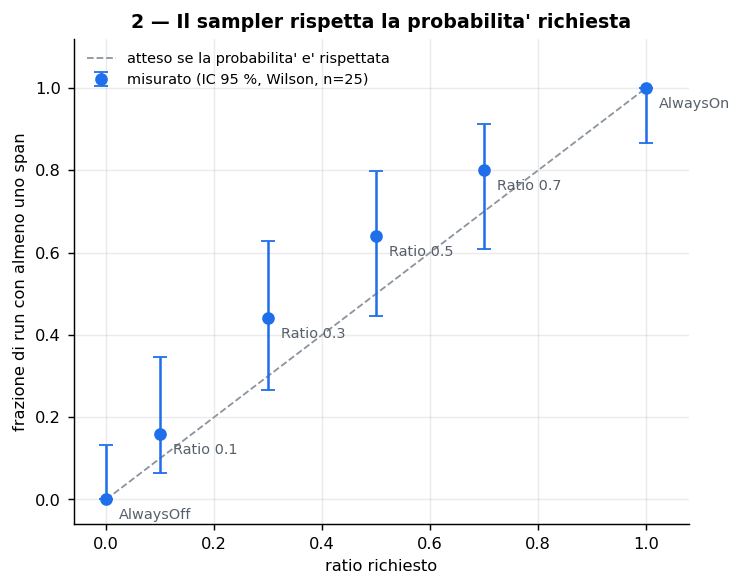
\includegraphics[width=0.62\textwidth]{../2-DoE/figures/02_sampling_fraction.png}
\caption{Frazione di esecuzioni campionate in funzione della proporzione richiesta; barre di
incertezza al 95\,\% su 25 ripetizioni per configurazione.}
\label{fig:02}
\end{figure}

La Figura~\ref{fig:02} completa il quadro e va letta insieme alla precedente. La frazione di
esecuzioni effettivamente campionate segue fedelmente la proporzione richiesta, e ogni intervallo
di confidenza contiene il valore nominale. Il meccanismo, dunque, \textbf{funziona correttamente};
ci\`o che non \`e adeguato \`e la granularit\`a alla quale opera.

\textbf{Conseguenza operativa.} Impostare una proporzione di campionamento pari a 0.1 non significa
``conserva il 10\,\% degli elementi'': significa ``scarta l'intera esecuzione, task critico
compreso, con probabilit\`a del 90\,\%''. Nei nostri dati, a tale proporzione, in 21 esecuzioni su
25 \textbf{non esiste alcuna traccia del task critico}. In un sistema a criticit\`a mista questo \`e
il comportamento meno desiderabile fra quelli possibili: la riduzione del volume di telemetria,
che \`e un'esigenza legittima, si ottiene sacrificando in modo indiscriminato proprio le
informazioni che si vorrebbero preservare. \`E la constatazione da cui muove la proposta esposta
nella \S6.

Sul piano temporale, l'esperimento non evidenzia differenze: il budget per iterazione risulta pari
a 9991\us{} in tutte e sei le configurazioni, campionamento disattivato compreso. Il confronto pi\`u
pulito \`e interno alle configurazioni proporzionali, dove le esecuzioni si dividono in campionate
e scartate in base al solo esito del sorteggio, a parit\`a di eseguibile e configurazione: i due
gruppi presentano lo stesso budget mediano, con differenza nulla entro la risoluzione della misura.

\subsection{Esperimento 3: la modalit\`a di consegna determina il costo}

\begin{figure}[h]\centering
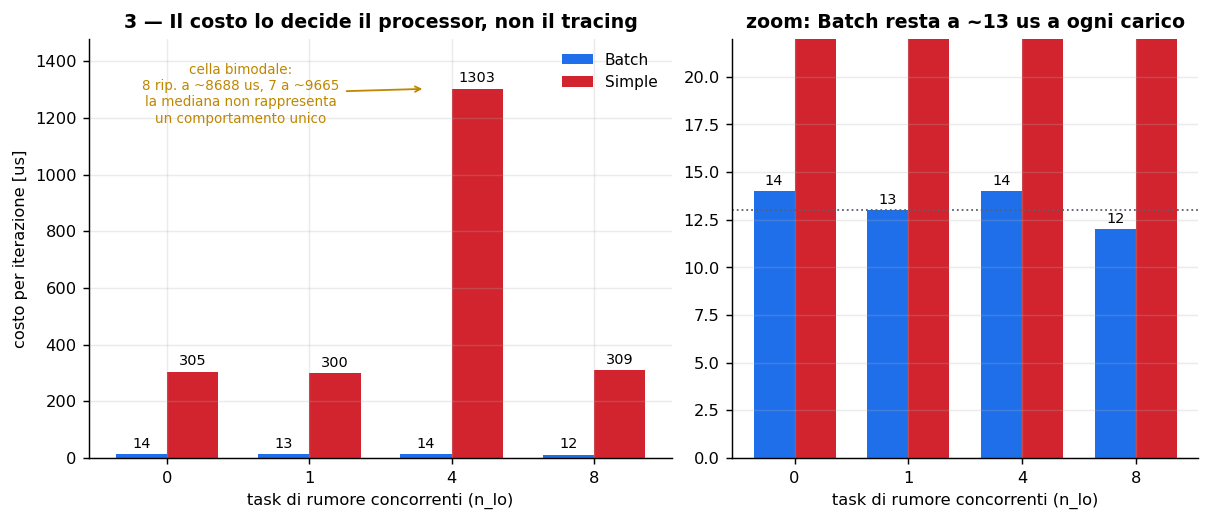
\includegraphics[width=\textwidth]{../2-DoE/figures/03_overhead_processor.png}
\caption{Costo per iterazione a carico crescente, rispetto alla condizione di controllo senza
tracciamento. A destra la stessa grandezza con scala espansa.}
\label{fig:03}
\end{figure}

La Figura~\ref{fig:03} riporta il costo per iterazione delle due modalit\`a di consegna, misurato
rispetto alla condizione di controllo allo stesso livello di carico. La consegna differita si
mantiene stabile fra 12 e 14\us{} a ogni livello di carico, in accordo con il valore ottenuto
nell'Esperimento 1. La consegna immediata costa circa \textbf{300\us}: ventitr\'e volte tanto, pari
al 3\,\% del periodo e al \textbf{15\,\% del lavoro utile}.

Il risultato sposta il baricentro delle conclusioni: non \`e la \emph{quantit\`a} di telemetria a
determinare il costo, ma il \emph{modo} in cui viene consegnata. A parit\`a di granularit\`a
massima, e quindi di numero di elementi prodotti, il costo per il task critico varia di oltre un
ordine di grandezza a seconda di questa sola scelta.

\emph{Un'avvertenza sulla lettura della figura.} La barra relativa a quattro task di disturbo
riporta un valore di 1303\us, segnalato nella figura stessa: quella configurazione presenta un
comportamento bimodale, con otto ripetizioni raggruppate attorno a un valore e sette attorno a un
altro, e la mediana cade sul primo gruppo. Il valore non va quindi interpretato come un costo
maggiore a quel livello di carico, e la non monotonia rispetto agli otto task di disturbo \`e solo
apparente. Il costo attribuibile alla consegna immediata resta quello indicato di circa 300\us;
l'origine del secondo comportamento non \`e stata determinata ed \`e segnalata fra i limiti dello
studio.

\begin{figure}[h]\centering
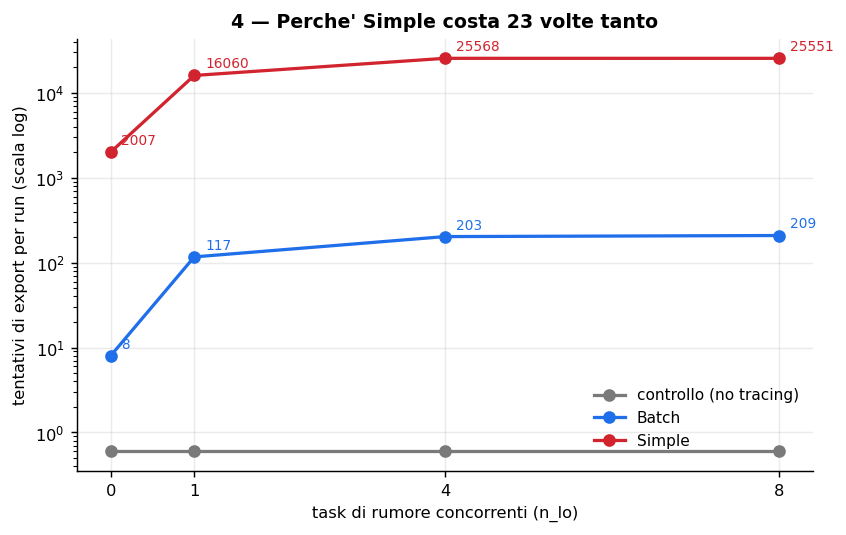
\includegraphics[width=0.72\textwidth]{../2-DoE/figures/04_export_attempts.png}
\caption{Numero di tentativi di trasmissione per esecuzione, in scala logaritmica.}
\label{fig:04}
\end{figure}

La Figura~\ref{fig:04} individua il meccanismo all'origine di tale divario, e non ne \`e una
semplice riformulazione. Nella modalit\`a immediata la trasmissione avviene \textbf{in modo sincrono,
all'interno del thread che ha appena prodotto l'elemento}, sotto un blocco condiviso fra tutti i
thread; nella modalit\`a differita gli elementi vengono accodati e trasmessi da un thread dedicato
a intervalli regolari. Il numero di tentativi di trasmissione per esecuzione passa da circa 230 a
oltre 25\,000: il task critico, nella prima modalit\`a, sostiene di persona il costo di ogni singola
trasmissione e concorre per il blocco condiviso con tutti gli altri thread.

Va sottolineato che nelle esecuzioni in esame \textbf{nessun servizio di raccolta era in ascolto}:
i tentativi di trasmissione falliscono immediatamente. Questa \`e la condizione \emph{pi\`u
favorevole} alla modalit\`a immediata; con un servizio realmente attivo, che accetta la connessione
e risponde, il divario sarebbe maggiore. I valori riportati vanno quindi intesi come un limite
inferiore.

\begin{figure}[h]\centering
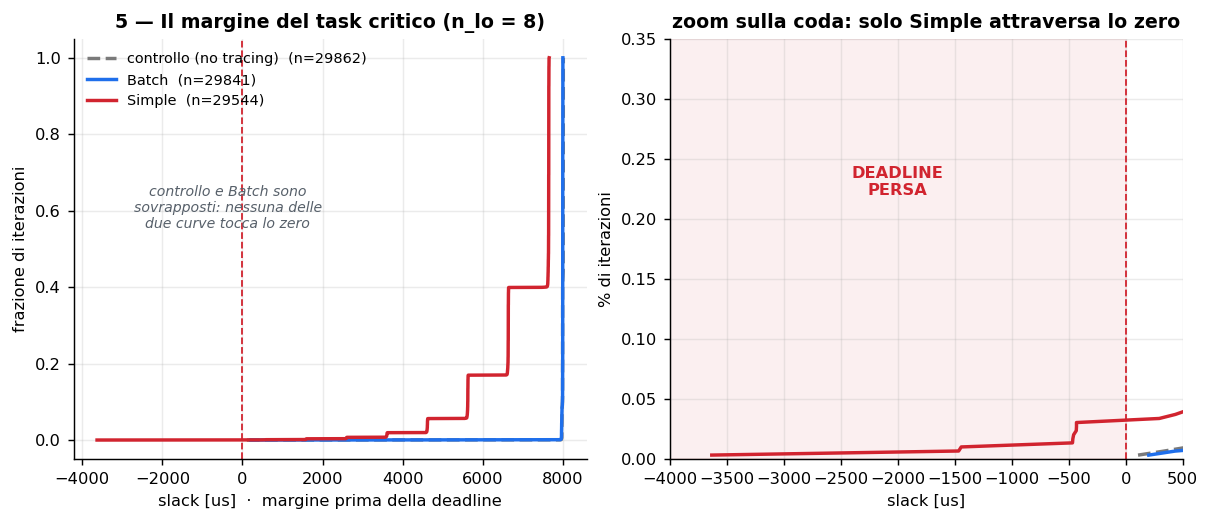
\includegraphics[width=\textwidth]{../2-DoE/figures/05_slack_distribution.png}
\caption{Distribuzione cumulativa del margine residuo del task critico al carico massimo; a destra
l'ingrandimento della coda.}
\label{fig:05}
\end{figure}

La Figura~\ref{fig:05} riporta la conseguenza sul rispetto delle scadenze. La condizione di
controllo e quella a consegna differita risultano sovrapposte e \textbf{non raggiungono mai lo
zero}: ogni iterazione si conclude con almeno 65\us{} di margine. La consegna immediata presenta
invece una coda che attraversa lo zero.

\`E l'unica figura che mostri il \emph{margine} anzich\'e il semplice conteggio dei fallimenti, e la
distinzione \`e sostanziale. Nove scadenze mancate su circa 29\,500 iterazioni (lo 0.03\,\%)
potrebbero apparire trascurabili in forma tabellare; la distribuzione mostra invece che il
comportamento \`e \textbf{qualitativamente diverso}, con una coda che si estende fino a
$-3631$\us: il task critico non sfora occasionalmente di poco, ma pu\`o eccedere la propria
scadenza di oltre un terzo del periodo. Si osserva inoltre che la separazione fra le due modalit\`a
\`e netta e priva di sovrapposizione, per cui la conclusione non dipende dalla scelta di una soglia.

Complessivamente, sulle 180 esecuzioni dell'esperimento le scadenze mancate sono 21, tutte nella
modalit\`a a consegna immediata e in presenza di carico concorrente; le condizioni di controllo e
quelle a consegna differita ne registrano \textbf{zero a qualunque livello di carico}. Le scadenze
mancate risultano distribuite uniformemente lungo l'esecuzione, e non concentrate in prossimit\`a
del termine: non sono quindi riconducibili alla fase di chiusura del programma.

Un'ulteriore osservazione riguarda la robustezza. Nella modalit\`a a consegna immediata, in presenza
di pi\`u thread, una frazione rilevante delle esecuzioni termina in modo anomalo al momento della
chiusura, con probabilit\`a crescente al crescere del numero di thread. Il fenomeno ha origine
nell'interazione fra il modo in cui il generatore di carico termina i propri thread e il fatto che
la funzione di consegna immediata sia dichiarata come non sollevante eccezioni: la terminazione
attraversa tale funzione e provoca l'arresto del processo. L'anomalia si manifesta \emph{dopo} che
tutti i dati sono stati scritti, e non compromette quindi le misure; \`e per\`o rilevante in
prospettiva applicativa, poich\'e in questa configurazione la scelta della modalit\`a di consegna
non degrada soltanto le prestazioni del task critico, ma pu\`o determinarne la terminazione.

\subsection{Sintesi dei risultati}

\begin{table}[h]\centering\small
\begin{tabular}{p{6.4cm}p{8.2cm}}
\toprule
\textbf{domanda} & \textbf{risposta sperimentale} \\
\midrule
La pipeline di telemetria prioritizza i task critici? &
\textbf{No.} La decisione di campionamento \`e presa per traccia e non per task: zero esecuzioni
parziali su 150. Ridurre il volume significa perdere anche il task critico. \\
\addlinespace
Quanto costa il monitoraggio al task critico? &
Circa 14\us{} per iterazione con consegna differita, a qualunque livello di carico; circa 300\us{}
con consegna immediata, pari al 15\,\% del lavoro utile. \\
\addlinespace
Il monitoraggio compromette il rispetto delle scadenze? &
Solo con consegna immediata e carico concorrente: 21 scadenze mancate, con margini fino a
$-3631$\us. Con consegna differita, nessuna. \\
\addlinespace
La granularit\`a del tracciamento \`e il fattore determinante? &
No: incide per 14\us{} soltanto al livello massimo. Il fattore determinante \`e la modalit\`a di
consegna. \\
\bottomrule
\end{tabular}
\caption{Sintesi delle evidenze raccolte.}
\end{table}

\subsection{Limiti dello studio}

\textbf{Assenza di un servizio di raccolta.} Tutte le esecuzioni sono state condotte senza un
servizio in ascolto. Come osservato, ci\`o rende i costi misurati un limite inferiore.

\textbf{Configurazione con comportamento bimodale.} Una delle dodici configurazioni
dell'Esperimento 3 presenta due comportamenti distinti fra le ripetizioni, per i quali non \`e stata
individuata una spiegazione; il dato \`e stato riportato con l'avvertenza corrispondente anzich\'e
essere sintetizzato in un valore unico.

\textbf{Piattaforma singola.} Le misure provengono da un solo sistema, con quattro core fisici e un
inviluppo termico limitato. I valori assoluti non sono trasferibili ad altro hardware; i confronti
fra configurazioni, condotti a parit\`a di ogni altra condizione, lo sono.
